\documentclass[11pt]{beamer}
\usetheme{Madrid}
\usepackage[utf8]{inputenc}

 \usepackage[english]{babel}

\usepackage{amsmath}
\usepackage{amsfonts}
\usepackage{amssymb}
\usepackage{graphicx}
\DeclareMathOperator {\argmin}{argmin}

\author{Feichun Yang}
\title{Model Selection with $AIC_c$}
% Informe o seu email de contato no comando a seguir
% Por exemplo, alcebiades.col@ufes.br
%\setbeamercovered{transparent} 
\setbeamertemplate{navigation symbols}{} 
\logo{\includegraphics[scale=0.08]{imagens/logomarca_profmat.png}} 
\institute[]{SYRACUSE UNIVERSITY} 
\date{\today} 
%\subject{}

% ---------------------------------------------------------
% Selecione um estilo de referência
\bibliographystyle{apalike}

%\bibliographystyle{abbrv}
%\setbeamertemplate{bibliography item}{\insertbiblabel}
% ---------------------------------------------------------

% ---------------------------------------------------------
% Incluir os slides nos quais as referências foram citadas
%\usepackage[brazilian,hyperpageref]{backref}

%\renewcommand{\backrefpagesname}{Citado na(s) página(s):~}
%\renewcommand{\backref}{}
%\renewcommand*{\backrefalt}[4]{
%	\ifcase #1 %
%		Nenhuma citação no texto.%
%	\or
%		Citado na página #2.%
%	\else
%		Citado #1 vezes nas páginas #2.%
%	\fi}%
% ---------------------------------------------------------

\begin{document}

\begin{frame}
\titlepage
\end{frame}

\begin{frame}{Outline}
\tableofcontents 
\end{frame}

\section{Summary of the Article}

\begin{frame}{Kullback-Leibler Discrepancy}
    \textbf{KL information} is a measure of discrepancy between the operating and approximating models.
     \begin{block}{Definition 1.1.1}
        \begin{equation}
        \Delta (\theta, \sigma^2) = E_F(-2\log g_{\theta, \sigma^2}(y))
        \end{equation}
        $F$: the operating model, $g_{\theta, \sigma^2}(y)$: the likelihood function under the approximating model
    \end{block}
    Goal: Find the competing approximating family which minimizes $E_F(\Delta (\hat{\theta}, \hat{\sigma}^2))$, where $\hat{\theta}$ and $\hat{\sigma}^2$ are MLE of $\theta$ and $\sigma^2$ in the approximating family.\\  
    Thus, we want to find the unbiased estimator of $E_F(\Delta (\hat{\theta}, \hat{\sigma}^2))$.\cite{hurvich1989regression}
\end{frame}

\begin{frame}{Akaike Information Criterion}
     Akaike information criterion, \textbf{AIC}(Akaike, 1973) is one of the selection methods for regression and autoregression model selection problems.\cite{seber2012linear}
     \begin{block}{Definition 1.1.2}
        \begin{equation}
        \label{}
        AIC = -2\log g_{\hat{\theta}, \hat{\sigma}^2}(y) + 2r
        \end{equation}
    \end{block}
     It provides an asymptotically efficient selection of a finite dimensional approximating model when the true model is \textbf{infinite} dimensional.
        
\end{frame}

\begin{frame}{limitations of $AIC$}
However, when the dimension of the true model is \textbf{finite}, especially when $n$ is small, AIC has following shortcomings:\cite{hurvich1989regression}
\begin{enumerate}
    \item does not provide consistent model order selections\cite{hannan1979determination}.
    \item tends to overfit severely without strong restrictions on the maximum allowable dimensions of the candidate models(cut-offs).
\end{enumerate}
AIC becomes a strongly negatively biased estimate of the KL information as $m/n$ increasing, which leads to overfitting.
\end{frame}

\begin{frame}
    to find an unbiased estimator of $E_F(\Delta (\hat{\theta}, \hat{\sigma}^2))$, \textbf{AIC} can be rewritten as:
        \begin{equation}
        AIC = n(\log \hat{\sigma}^2+1)+2(m+1)
        \end{equation}
    By assuming that the approximating family includes the operating model, we can write $\mu$ as $\mu = h(\theta^*)$
    then 
    \begin{align}
        \frac{1}{\hat\sigma^2}\frac{n-m}{nm}(\mu-h(\hat\theta))^T(\mu-h(\hat\theta)) & \approx (\frac{n-m}{nm})\frac{1}{\hat\sigma^2}(\hat\theta-\theta^*)^TV^TV(\hat\theta-\theta^*) \\
        & \sim F(m, n-m)
     \end{align}
     Thus,$$E_F(\Delta (\hat{\theta}, \hat{\sigma}^2)) \approx E_F(n\log \hat\sigma^2)+n^2/(n-m-2)+nm/(n-m-2)$$
     
\end{frame}

\begin{frame}{Definition 1.1.3}
Then we get an approximately unbiased estimator of $E_F(\Delta (\hat{\theta}, \hat{\sigma}^2))$:
\begin{block}{$AIC_C$}
\begin{align}
    AIC_C &= n\log \hat\sigma^2 +n\frac{1+m/n}{1-(m+2)/n}\\
            &= AIC + \frac{2(m+1)(m+2)}{n-m-2}
\end{align}
\end{block}
\end{frame}

\begin{frame}{Improvements}
\begin{enumerate}
    \item $AIC_C$ is asymptotically efficient for regression and time series
    \item $AIC_C$ is unbiased for linear regression, and approximately unbiased for nonlinear regression and time series models.
    \item The bias decreases without any increase in variance.
    \item A maximum model order cut-off is not needed for $AIC_C$
\end{enumerate}
\end{frame}

\begin{frame}{Simulation Results}
The small-sample performance of various selection criteria in the linear
regression case:
    \begin{figure}[htb]
        \centering
        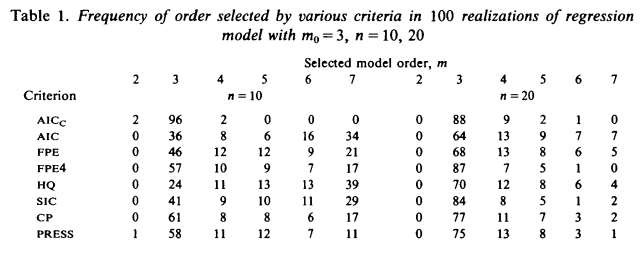
\includegraphics[width=1\textwidth]{drive.google.com_file_d_15QZ0OuCAEpjZRO1xj0kAWJdI5QHMy-5W_view (1)}
        \medskip
    \end{figure}
\end{frame}

\begin{frame}{Simulation Results}
\begin{figure}[htb]
        \centering
        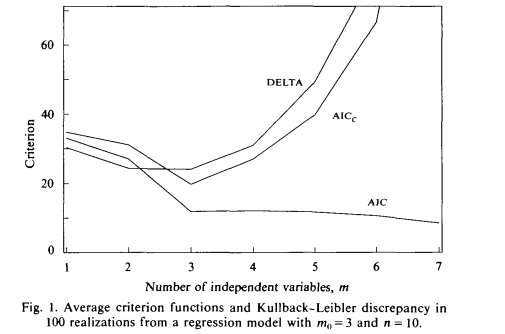
\includegraphics[width=1\textwidth]{drive.google.com_file_d_15QZ0OuCAEpjZRO1xj0kAWJdI5QHMy-5W_view (2)}
        \medskip
    \end{figure}

\end{frame}

\begin{frame}{Autoregression}
\begin{block}
$$AIC = n(\log \hat P_m +1)+2(m+1)$$
\end{block}

\begin{block}
$$AIC_C = n\log \hat P_m +n\frac{1+m.n}{1-(m+2)/n}$$
\end{block}

\end{frame}

\begin{frame}{Simulation Results}
\begin{figure}[htb]
        \centering
        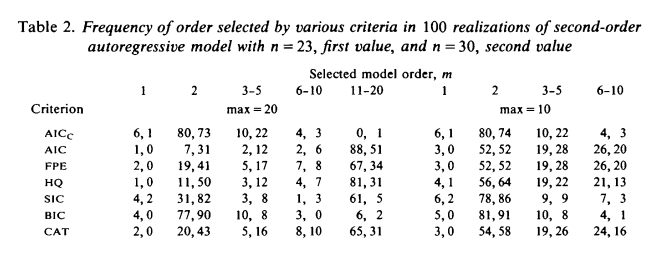
\includegraphics[width=1\textwidth]{drive.google.com_file_d_15QZ0OuCAEpjZRO1xj0kAWJdI5QHMy-5W_view (3)}
        \medskip
    \end{figure}

\end{frame}

\begin{frame}{Simulation Results}
\begin{figure}[htb]
        \centering
        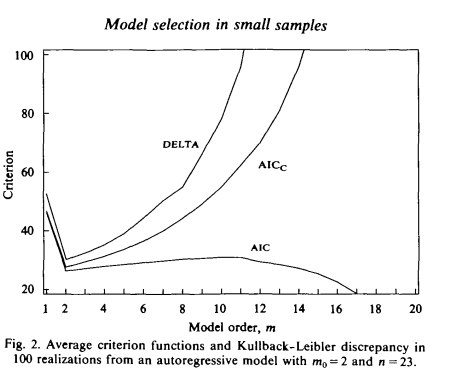
\includegraphics[width=0.7\textwidth]{drive.google.com_file_d_15QZ0OuCAEpjZRO1xj0kAWJdI5QHMy-5W_view (4)}
        \medskip
    \end{figure}
\end{frame}

\begin{frame}{Simulation Results}
\begin{figure}[htb]
        \centering
        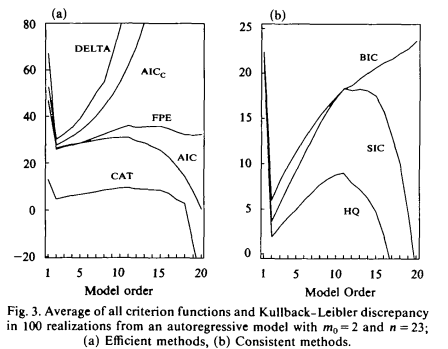
\includegraphics[width=0.7\textwidth]{drive.google.com_file_d_15QZ0OuCAEpjZRO1xj0kAWJdI5QHMy-5W_view (5)}
        \medskip
    \end{figure}
\end{frame}

\section{Application of $AIC_c$}
\begin{frame}{Model Selection for Linear Regression Model}
Full model:
$$Y = \beta_0 +\beta_1x_1 +\cdots +\beta_mx_m+\epsilon$$
Try all possible combinations of the $x$'s.\\

Selection Criteria:\\
Information based criteria:\\
\begin{itemize}
    \item $AIC = \min \log(RSS_p/n)+\frac{2p}{n}$
    \item $BIC = \min \log(RSS_p/n)+\frac{\log(n)p}{n}$
\end{itemize}
$$AIC_C = AIC + \frac{2(m+1)(m+2)}{n-m-2}$$
\end{frame}

\begin{frame}{Data Simulation}
Assume the true model is
    $Y = \mu + \epsilon$,
where $\epsilon\sim N(0,\sigma_0^2)$, and $\mu = X_0\theta_0$.
\begin{figure}[htb]
        \centering
        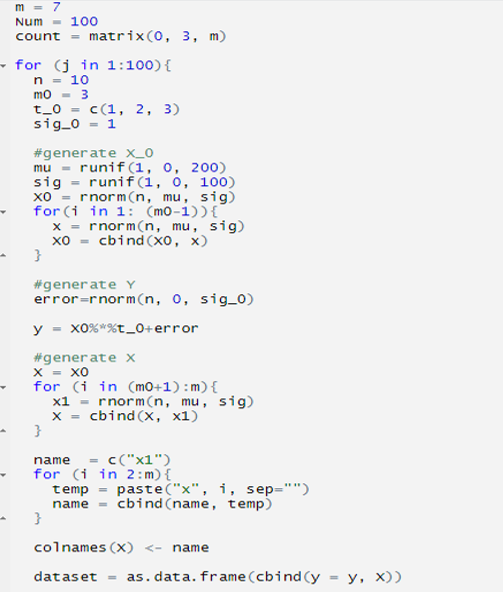
\includegraphics[width=0.7\textwidth]{Picture1}
        \medskip
    \end{figure}

\end{frame}

\begin{frame}{Code Rewriting}
\begin{figure}[htb]
        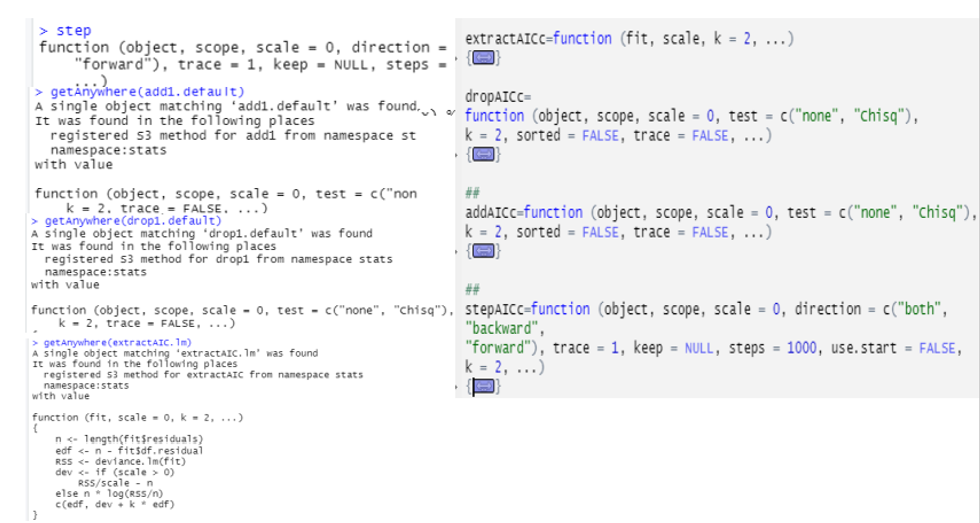
\includegraphics[width=1.1\textwidth]{Picture2}
        \medskip
    \end{figure}
 
\end{frame}

\begin{frame}
\begin{figure}[htb]
        \centering
        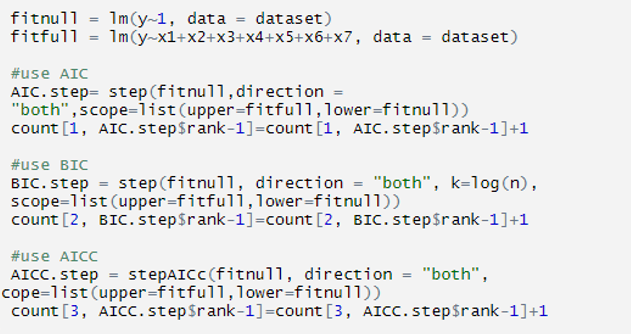
\includegraphics[width=0.7\textwidth]{Picture3}
        \medskip
    \end{figure}
\end{frame}

\begin{frame}{Results}
\begin{center}
\begin{tabular}{ c | c c c c c c c}
\hline
 \multicolumn{8}{c}{n = 10, $m_0$= 3} \\
 \hline
    m  & 1 & 2 & 3($m_0$) & 4 & 5 & 6 & 7\\
    \hline
 $AIC$ & 1 & 1 & 18 & 22 & 28 & 11 &18\\ 
 $BIC$ & 1 & 1 & 21 & 27 & 22 & 11 & 16 \\  
 $AIC_C$ & 6 & 2 & 86 & 4 & 0 & 0 & 0 
\end{tabular}
\end{center}
 \begin{itemize}
     \item $AIC_C$ provides the best selection among $m$ over $AIC$ and $BIC$
     \item $AIC$ and $BIC$ tends to select model with larger $m$.
 \end{itemize}

 \end{frame}

\begin{frame}
\begin{center}
\begin{tabular}{ c | c c c c c c c}
\hline
 \multicolumn{8}{c}{n = 50, $m_0$= 3} \\
 \hline
    m  & 1 & 2 & 3($m_0$) & 4 & 5 & 6 & 7\\
    \hline
 $AIC$ & 0 & 0 & 52 & 36 & 7 & 4 &1\\ 
 $BIC$ & 0 & 0 & 81 & 17 & 1 & 1 & 0 \\  
 $AIC_C$ & 0 & 0 & 63 & 31 & 4 & 2 & 0 
\end{tabular}
\end{center}
 \begin{itemize}
    \item $BIC$ provides the best selection when $n$ is large.
     \item $AIC_C$ performs similarly as $AIC$.
 \end{itemize}
 
\end{frame}



\section{Reference}
\begin{frame}{Reference}
    \bibliography{referencias}
\end{frame}


\end{document}